\section{Inserting Vertices}
\label{sect:inserting-vertices}

When a new cluster appears in our underlying data set, we want to add a new vertex to the cluster graph and have that change translate to an existing polygonal dual thereof.
We distinguish between adding a new vertex in an internal face and adding a new vertex in the outer face because slightly different rules apply.



\paragraph{Inserting Vertices Inside}

All internal faces of the filtered cluster graph \clustergraph{t} are triangles.
If we add a vertex in one of the triangular faces, we must also add edges to the three vertices bounding the face without introducing edge crossings to preserve the graph's internal triangulatedness.
\Cref{fig:insert-vertex-example-inside} shows an example of a valid vertex insertion into an internal face.

\begin{figure}[H]
	\centering
	\subfigure[]{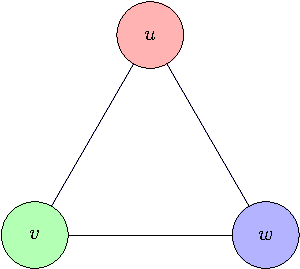
\includegraphics[height=28mm]{Resources/InsertVertex-Example-Inside-1.pdf}}
	\quad
	\subfigure[]{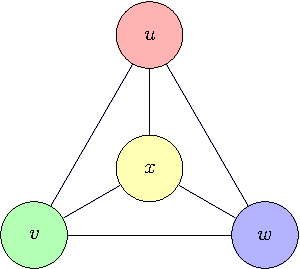
\includegraphics[height=28mm]{Resources/InsertVertex-Example-Inside-2.pdf}}
	\qquad
	\subfigure[]{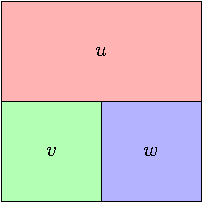
\includegraphics[height=28mm]{Resources/InsertVertex-Example-Inside-3.pdf}}
	\quad
	\subfigure[]{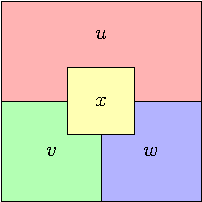
\includegraphics[height=28mm]{Resources/InsertVertex-Example-Inside-4.pdf}}
	\caption{A cluster graph and a polygonal dual thereof, before (a, c) and after (b, d) inserting the vertex $x$ in the triangular face $uvw$.}
	\label{fig:insert-vertex-example-inside}
\end{figure}

Let $u$, $v$, and $w$ be the vertices bounding an internal face of the cluster graph in counterclockwise order and let $x$ be the new vertex we want to add inside said face.

Let $p_{uvw}$ be the vertex of the map \initmap{t} that is common to faces $u$, $v$, and $w$.
Also, let $p_{uv}$, $p_{vw}$, and $p_{wu}$ denote the subdivision vertices on the boundary of these faces that are incident to $p_{uwv}$, as illustrated in \cref{subfig:insert-vertex-illustration-1}.
If one of the boundaries consist of only one edge, we subdivide the edge at its midpoint first.

\begin{figure}[H]
	\centering
	\subfigure[]{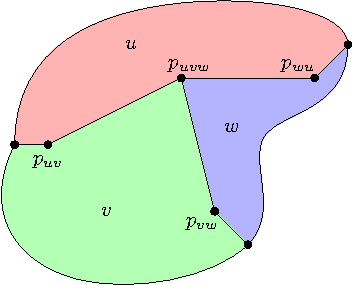
\includegraphics[width=45mm]{Resources/InsertVertex-Illustration-1.pdf}\label{subfig:insert-vertex-illustration-1}}
	\quad
	\subfigure[]{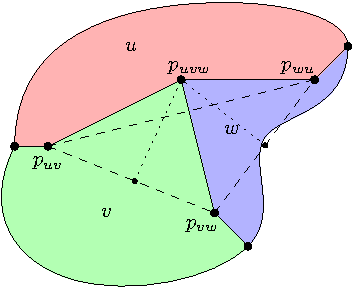
\includegraphics[width=45mm]{Resources/InsertVertex-Illustration-2.pdf}\label{subfig:insert-vertex-illustration-2}}
	\quad
	\subfigure[]{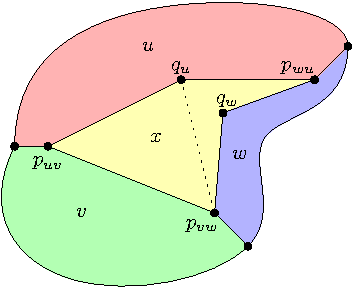
\includegraphics[width=45mm]{Resources/InsertVertex-Illustration-3.pdf}\label{subfig:insert-vertex-illustration-3}}
	\caption{Inserting an internal face $x$ at the point where three faces $u,v,w$ meet.}
	\label{fig:insert-vertex-illustration}
\end{figure}

We then want to remove the vertex $p_{uvw}$ along with its incident edges and insert edges between the subdivision vertices instead to bound a new face for $x$, as illustrated by the dashed lines in \cref{subfig:insert-vertex-illustration-2}.
Doing so naïvely may introduce edge crossings, though, and we generally need to add bends in the form of subdivision vertices to those edges.

To determine if we need a bend and where to position it, we distinguish three cases, all of which are illustrated in \cref{subfig:insert-vertex-illustration-3}.
Let $(a,b,c)$ be a rotation of $(u,v,w)$, \ie{}, $(a,b,c) \in \{(u,v,w), (v,w,u), (w,u,v)\}$.
Then the three cases are the following:
%
\begin{itemize}
\item If we can place an edge between $p_{ab}$ and $p_{bc}$ without introducing an edge crossing, we do not need to bend the edge (face $v$ in \cref{subfig:insert-vertex-illustration-3}).
\item Otherwise, if the internal angle of face $a$ at $p_{abc}$, $\angle_{p_{ab}p_{abc}p_{bc}}$, is $180^\circ$ or more, we bend the edge using a subdivision vertex $q_a$ at $p_{abc}$.
(face $u$ in \cref{subfig:insert-vertex-illustration-3})
\item Otherwise, we do a binary search for a bend location in the form of a subdivision vertex $q_a$ on the outward-pointing bisector of the angle $\angle_{p_{ab}p_{abc}p_{bc}}$ (dotted lines in \cref{subfig:insert-vertex-illustration-2}).
We start at the point where the bisector intersects the line segment from $p_{ab}$ to $p_{bc}$ and keep dividing the remaining distance to $p_{abc}$ in half until we find a bend location for which the bent edge from $p_{ab}$ to $p_{bc}$ would not introduce edge crossings.
(face $w$ in \cref{subfig:insert-vertex-illustration-3})
\end{itemize}

Considering at most one of the internal angles at $p_{uvw}$ can be $180^\circ$ or more, we place at most one subdivision vertex there.
By removing the vertex $p_{uvw}$ and inserting the edges $\{p_{uv},p_{vw}\}$, $\{p_{vw},p_{wu}\}$, and $\{p_{wu},p_{uv}\}$, potentially with bends $q_v$, $q_w$, and $q_u$, we create an internal face for $x$ without introducing edge crossings.



\paragraph{Inserting Vertices Outside}

Alternatively, we can add a new vertex in the outer face of the filtered cluster graph.
Such a vertex must be connected to at least two vertices on the outer face to preserve the graph's biconnectivity.
Its neighbors must also form a path on the original boundary of the cluster graph in order not to create holes and thereby violate its internal triangulatedness.

We restrict ourselves to adding new vertices in the outer face that are made incident to exactly two neighboring vertices here.
Additional edges can be inserted separately afterward, as discussed in \cref{sect:flipping-edges}.
Let $\{u,v\}$ be an edge on the outer face.
Then we support adding a new vertex $x$ in the outer face and connecting it to both $u$ and $v$.
\Cref{fig:insert-vertex-example-outside} shows an example of a valid vertex insertion into the outer face.

\begin{figure}[H]
	\centering
	\subfigure[]{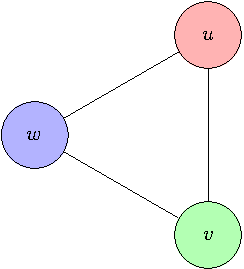
\includegraphics[height=28mm]{Resources/InsertVertex-Example-Outside-1.pdf}}
	\quad
	\subfigure[]{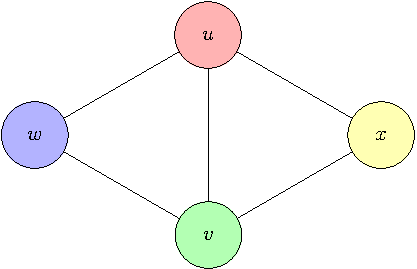
\includegraphics[height=28mm]{Resources/InsertVertex-Example-Outside-2.pdf}}
	\qquad
	\subfigure[]{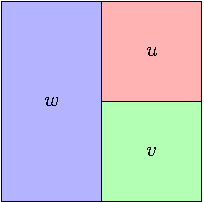
\includegraphics[height=28mm]{Resources/InsertVertex-Example-Outside-3.pdf}}
	\quad
	\subfigure[]{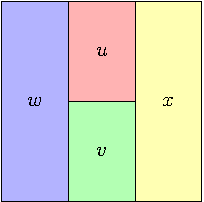
\includegraphics[height=28mm]{Resources/InsertVertex-Example-Outside-4.pdf}}
	\caption{A cluster graph and a polygonal dual thereof, before (a, c) and after (b, d) inserting the vertex $x$ on the outer face and connecting it to $u$ and $v$.}
	\label{fig:insert-vertex-example-outside}
\end{figure}

This operation is a special case of the vertex insertion discussed above:
In the polygonal dual, instead of creating a new face between three internal faces, we need to create a new face between two internal faces and the implicit outer face.

Recall that the polygonal dual is a subdivision of the augmented dual $(\clustergraph{t})^+$ of the cluster graph \clustergraph{t}.
In the construction of the augmented dual from \cref{def:augmented-dual}, we insert a helper vertex incident to all vertices on the outer face of the primal graph and then form the regular dual.
That is why the polygonal dual has an internal face for each of the vertices in $(\clustergraph{t})^+$.
The polygonal dual also has an implicit outer face \emdash{} an ocean in the context of maps \emdash{} that corresponds to the helper vertex inserted during the construction of the augmented dual, as illustrated in \cref{fig:insert-vertex-duality}.

\begin{figure}[H]
	\centering
	\subfigure[]{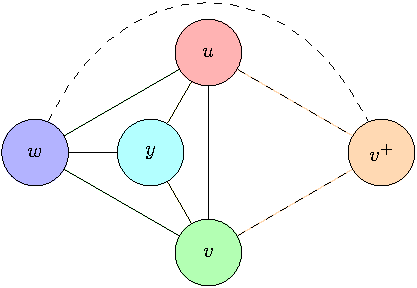
\includegraphics[height=28mm]{Resources/InsertVertex-Duality-1.pdf}}
	\quad
	\subfigure[]{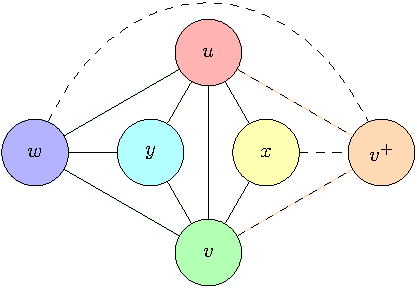
\includegraphics[height=28mm]{Resources/InsertVertex-Duality-2.pdf}}
	\qquad
	\subfigure[]{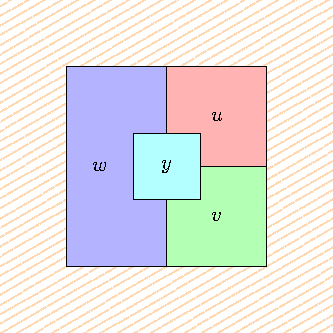
\includegraphics[height=28mm]{Resources/InsertVertex-Duality-3.pdf}}
	\quad
	\subfigure[]{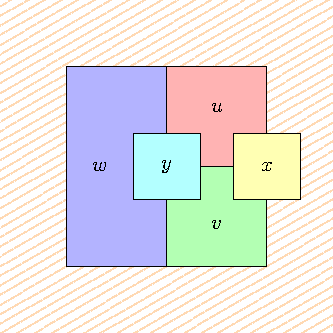
\includegraphics[height=28mm]{Resources/InsertVertex-Duality-4.pdf}}
	\caption{A cluster graph and a polygonal dual thereof with explicit helper vertex $v^+$ and outer face, before (a, c) and after (b, d) inserting the vertex $x$ in the triangle $u$ and $v$ form with $v^+$.}
	\label{fig:insert-vertex-duality}
\end{figure}

Also recall that the cluster graph with this helper vertex is triangulated.
Two arbitrary adjacent vertices on the outer face of \clustergraph{t} form a triangular face with the helper vertex $v^+$.
As a result, inserting a new vertex $x$ in the outer face as described above is equivalent to inserting $x$ in the triangular face $u$ and $v$ form with the helper vertex $v^+$, or, in the dual, inserting a face at the point where the faces $u$ and $v$ meet the implicit outer face.

The construction outlined above translates 1-to-1 to inserting a vertex in the outer face, except one of the three neighboring faces is the implicit outer face.
